\subsection{Cross-Database Experiments}

I firstly pre-trained my models on the Finger Knuckle V1 Database, and then fine-tuned models on the Finger Knuckle V3 Database (with deformable). I use these kind training method, and use these models to test performance on the Index Finger Knuckle of Hand Dorsal Image and Tsinghua Finger Knuckle Database as a cross database experiment. The label in the finger curve, the content in parentheses indicates the training samples. Such as RFN-WS(1-104), it uses 1-104 subjects of Finger Knuckle V3 Database to train models. Updated ROC Curve and CMC Curve with RFNet, EfficientNet and DeConvRFNet. For the ROC curve, I add EfficientNetV2-S model performance.

\subsubsection{Index Finger Knuckle of Hand Dorsal Image}

\begin{figure}[H]
	\centering
	\begin{subfigure}[b]{0.45\linewidth}
		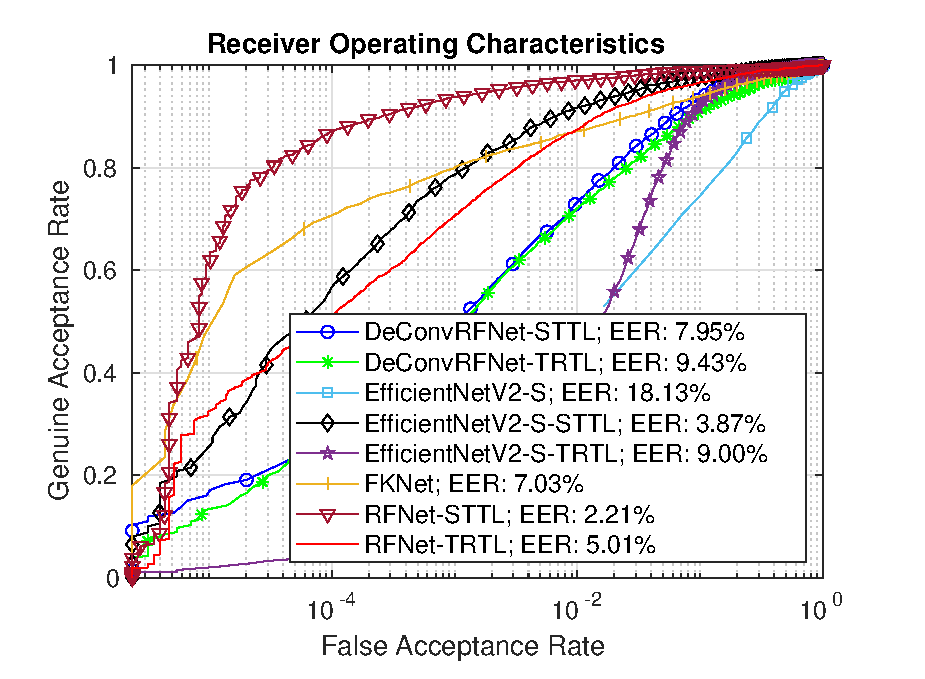
\includegraphics[width=\linewidth]{Figures/crosshd-roc_compare_new.eps}
	\end{subfigure}
    \begin{subfigure}[b]{0.45\linewidth}
		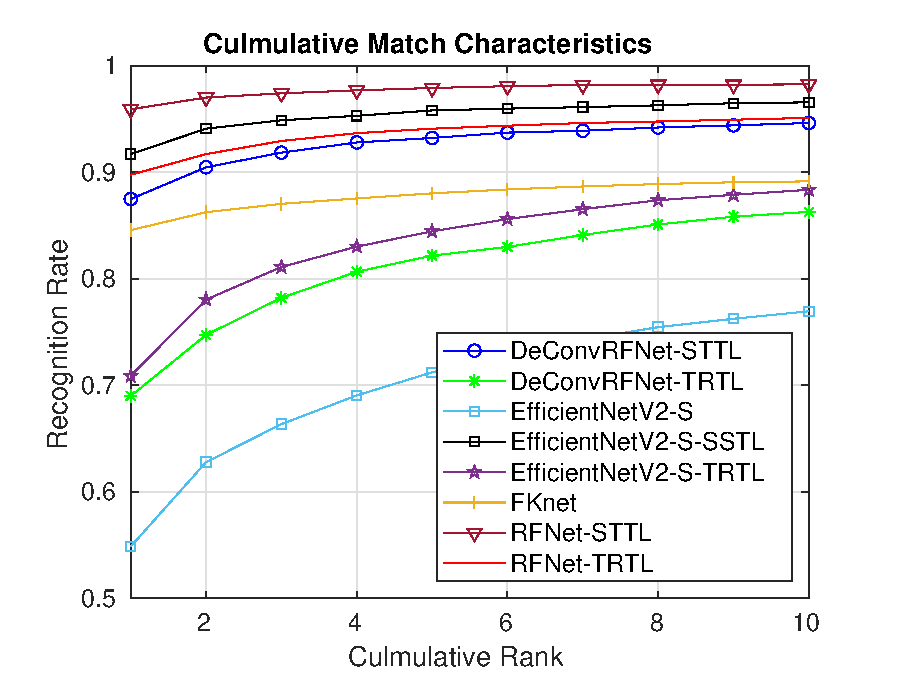
\includegraphics[width=\linewidth]{Figures/crosshd-cmc_compare_new.eps}
	\end{subfigure}
\end{figure}

The database totally has 712 subjects, and each subject has 5 samples. Therefore, it will have $712*5$ genuine matching scores and $712*711*5$ imposter matching scores. From the cure, the performance of RFN-WS and RFN-WRS is similar, and the RFN-WS is slightly better than RFN-WRS while using the same training samples. Updated ROC Curve and CMC Curve with RFNet, EfficientNet and DeConvRFNet. For the ROC curve, I add EfficientNetV2-S model performance.

\subsubsection{Middle Finger Knuckle of Hand Dorsal Image}
\begin{figure}[H]
	\centering
	\begin{subfigure}[b]{0.45\linewidth}
		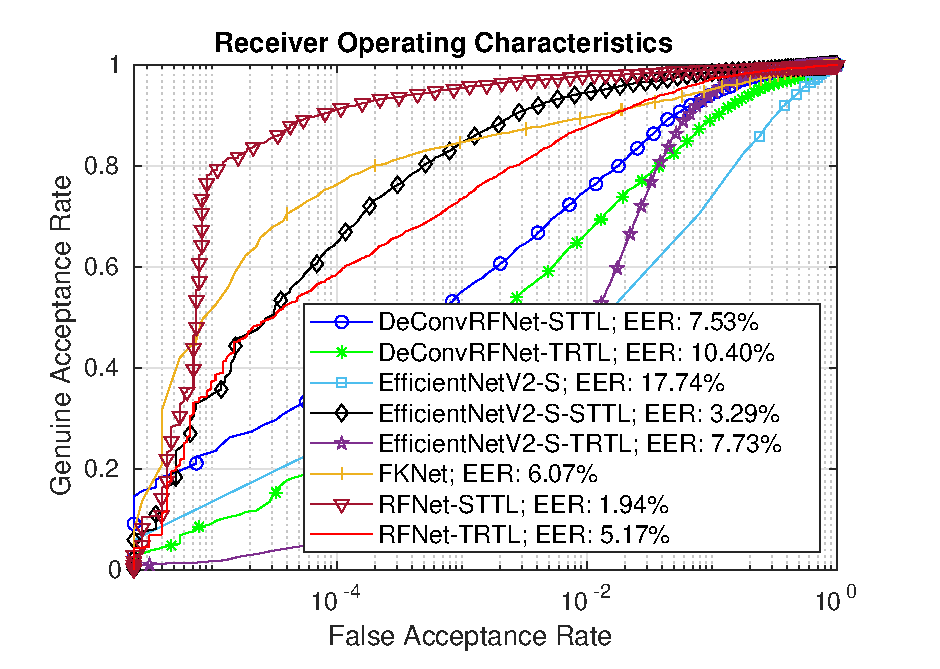
\includegraphics[width=\linewidth]{Figures/crosshd-middle-roc_compare_new.eps}
	\end{subfigure}
    \begin{subfigure}[b]{0.45\linewidth}
		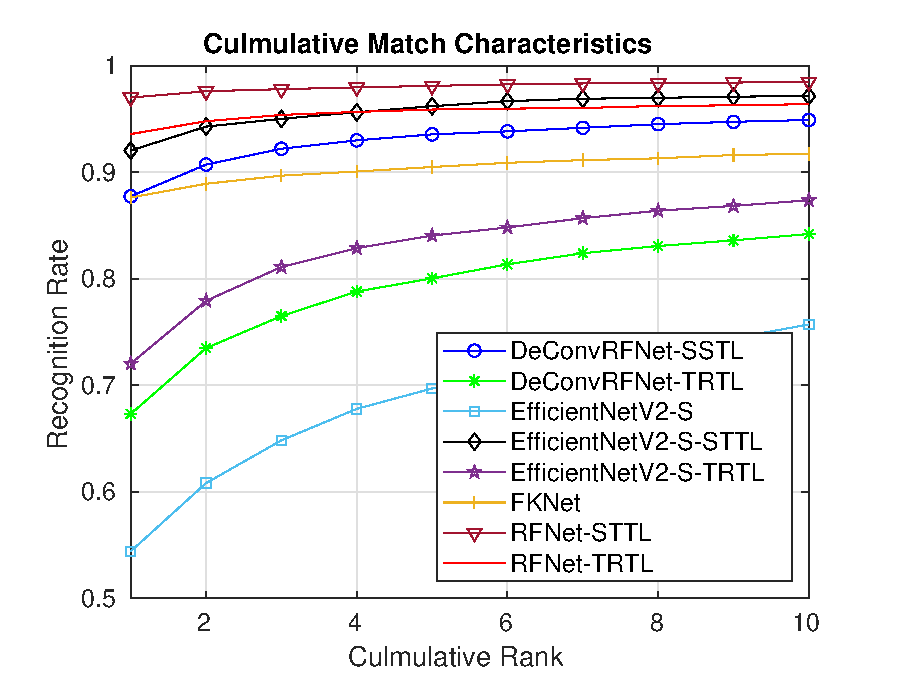
\includegraphics[width=\linewidth]{Figures/crosshd-middle-cmc_compare_new.eps}
	\end{subfigure}
\end{figure}


\subsubsection{Tsinghua Finger Knuckle Database}
\begin{figure}[H]
	\centering
	\begin{subfigure}[b]{0.45\linewidth}
		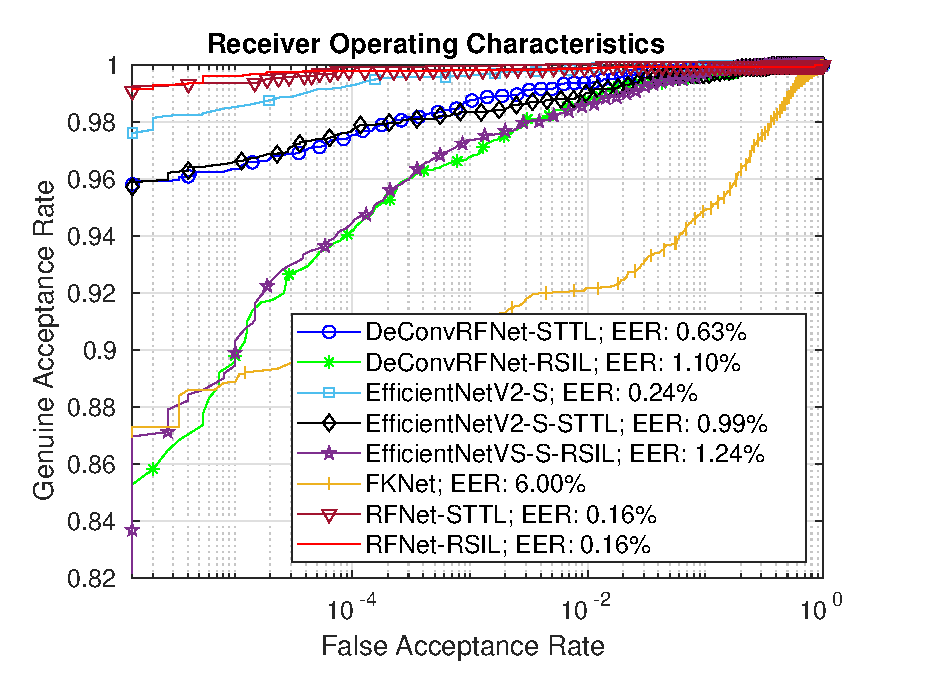
\includegraphics[width=\linewidth]{Figures/crossthu-roc_compare_new.eps}
	\end{subfigure}
    \begin{subfigure}[b]{0.45\linewidth}
		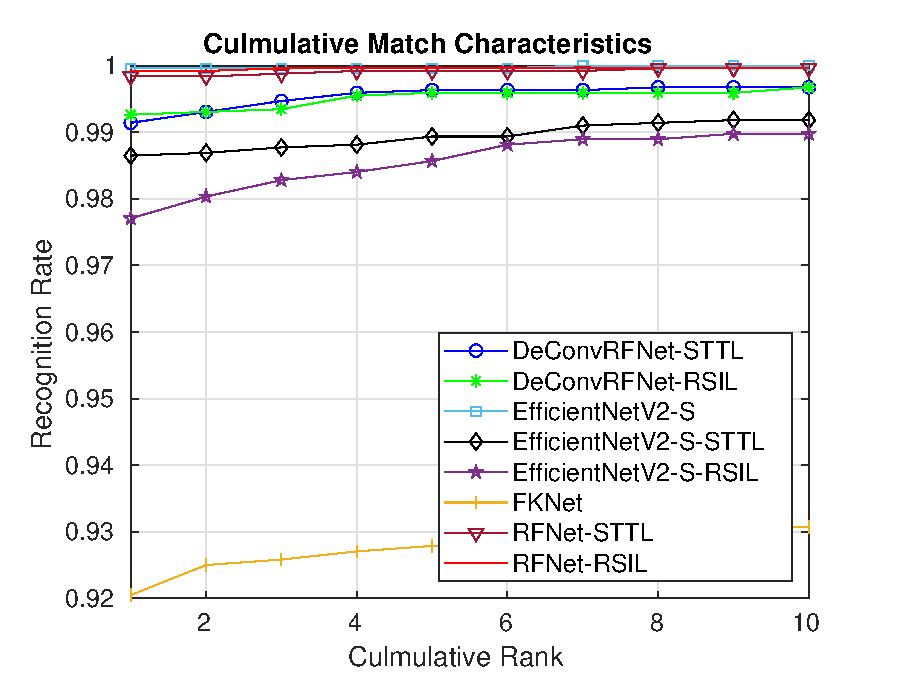
\includegraphics[width=\linewidth]{Figures/crossthu-cmc_compare_new.eps}
	\end{subfigure}
\end{figure}

The database has 610 subjects, and each subject can offer 4 samples. Then as the cross database experiment, it will have $610*4$ genuine matching scores and $610*609*4$ imposter matching scores. In this database, all models can get very high matching performance from the table and figure.

\subsection{Discussion}
From these experiment results, we can see that EfficientV2-S model is better than FKNet in some dataset. Becuase EfficientNetV2 model use MBConv as a block unit for replacing residual block. As for MBConv block, it use depthwise convolutions to decrease training weights and use Squeeze-Excited block as channel tranfomer. Meanwhile, the depth of EfficientNetV2-S is deeper than the FKNet.

There is another conclusion is that TRTL generalization ablity is lower thant STTL loss from the cross database experiment. But in the within database experiment, these model with TRTL loss is better thant STTL loss.

..............
